\documentclass[full-course-notes.tex]{subfiles}

\begin{document}
\lecturemeta{4}
  {Regular Languages vs.\ Non-Regular Languages; Regular Expressions and Regular Definitions}
  {CLO 1}
  {\S3.3 (Specification of Tokens: Strings, Languages, Operations, Regular Expressions, Regular Definitions, Extensions)}
  {[PP] Programming Language Pragmatics \S3.3}
\lecshort{Regular Expressions \& Definitions}
\setcounter{section}{0}
\makelecturetitle

\begin{coreidea}[Lecture Roadmap]
\begin{enumerate}
  \item Strings, alphabets, and languages -- the formal vocabulary underneath ``pattern.''
  \item Operations on languages: union, concatenation, and closure.
  \item \textbf{Regular expressions}: the formal, inductive definition, plus many worked examples.
  \item \textbf{Regular definitions}: naming sub-expressions, culminating in DB's classic
  identifier and numeric-literal definitions.
  \item Extensions (\texttt{+}, \texttt{?}, character classes) -- convenience, not new power.
  \item \textbf{Regular vs.\ non-regular languages}: what a lexer's patterns fundamentally
  cannot express, and why that is exactly the job handed to the parser.
\end{enumerate}
Today makes ``pattern'' from Lecture 3 completely precise. Lectures 5--6 show \emph{how} a
machine matches a regular expression, via finite automata.
\end{coreidea}

\section{Strings, Alphabets, and Languages}

\dbtag Before regular expressions can be defined precisely, three primitive terms need to be
pinned down exactly as DB uses them.

\begin{defbox}{Alphabet, String, Language}
\begin{itemize}
  \item An \textbf{alphabet} $\Sigma$ is any finite set of symbols, e.g.\ $\{0,1\}$ or the set
  of ASCII characters.
  \item A \textbf{string} (or \emph{word}) over $\Sigma$ is a finite sequence of symbols drawn
  from $\Sigma$. The \textbf{empty string}, written $\varepsilon$, has length 0.
  \item A \textbf{language} over $\Sigma$ is simply \emph{any} set of strings over $\Sigma$ ---
  possibly infinite, possibly empty ($\emptyset$, the language with no strings at all, which is
  \emph{not} the same as $\{\varepsilon\}$, the language containing only the empty string).
\end{itemize}
\end{defbox}

\begin{examfocus}
$\emptyset$ and $\{\varepsilon\}$ are a classic confusion. $\emptyset$ contains \emph{zero}
strings; $\{\varepsilon\}$ contains \emph{one} string (the empty one). Keep them distinct.
\end{examfocus}

\subsection{Operations on Languages}

\dbtag Given two languages $L$ and $M$ over the same alphabet, DB defines four operations that
build new languages out of old ones. These four operations are the entire foundation regular
expressions are built from.

\begin{center}
\renewcommand{\arraystretch}{1.35}
\begin{tabularx}{\textwidth}{@{}l l X@{}}
\toprule
\textbf{Operation} & \textbf{Notation} & \textbf{Definition} \\
\midrule
Union & $L \cup M$ & $\{\, s \mid s \in L \text{ or } s \in M \,\}$ \\
Concatenation & $LM$ & $\{\, st \mid s \in L \text{ and } t \in M \,\}$ (paste a string from $L$
directly onto a string from $M$) \\
Kleene closure & $L^{*}$ & $\bigcup_{i=0}^{\infty} L^{i}$ -- zero or more strings from $L$,
concatenated (includes $\varepsilon$, from $L^0$) \\
Positive closure & $L^{+}$ & $\bigcup_{i=1}^{\infty} L^{i}$ -- one or more strings from $L$,
concatenated (excludes $\varepsilon$ unless $\varepsilon \in L$) \\
\bottomrule
\end{tabularx}
\end{center}

\begin{examplebox}{Worked Example: Letters and Digits}
Let $L = \{a, b, c, \dots, z, A, \dots, Z\}$ (the 52 letters) and $D = \{0, 1, \dots, 9\}$ (the
10 digits), each treated as a language of one-character strings.
\begin{itemize}
  \item $L \cup D$ -- every single letter \emph{or} single digit: 62 strings, each of length 1.
  \item $LD$ -- every string formed by one letter followed by one digit, e.g.\ \texttt{a5},
  \texttt{Z0} -- exactly $52 \times 10 = 520$ strings, each of length 2.
  \item $L^{4}$ -- every string of exactly 4 letters, e.g.\ \texttt{Test}, \texttt{abcd} --
  there are $52^{4}$ such strings in total.
  \item $L^{*}$ -- every string of letters of \emph{any} length, including $\varepsilon$ ---
  infinitely many strings.
  \item $L(L \cup D)^{*}$ -- one letter, followed by zero or more letters-or-digits. This is
  \emph{exactly} the language of identifiers in most C-like languages! We will turn this
  directly into a regular expression in \S3.
\end{itemize}
\end{examplebox}

\section{Regular Expressions}

\dbtag A \textbf{regular expression} is a compact notation for describing a language. DB
defines regular expressions \emph{inductively}: a small set of base cases, plus rules for
combining smaller regular expressions into bigger ones.

\begin{defbox}{Regular Expressions (Inductive Definition)}
Over alphabet $\Sigma$:
\begin{itemize}
  \item \textbf{Base case 1:} $\varepsilon$ is a regular expression; $L(\varepsilon) = \{\varepsilon\}$.
  \item \textbf{Base case 2:} for each symbol $a \in \Sigma$, $a$ is a regular expression;
  $L(a) = \{a\}$.
  \item \textbf{Inductive case (union):} if $r$ and $s$ are regular expressions, so is
  $r \mid s$, with $L(r \mid s) = L(r) \cup L(s)$.
  \item \textbf{Inductive case (concatenation):} if $r$ and $s$ are regular expressions, so is
  $rs$, with $L(rs) = L(r)L(s)$.
  \item \textbf{Inductive case (closure):} if $r$ is a regular expression, so is $r^{*}$, with
  $L(r^{*}) = (L(r))^{*}$.
  \item \textbf{Parenthesization:} if $r$ is a regular expression, so is $(r)$, with
  $L((r)) = L(r)$ -- used purely to control grouping/precedence.
\end{itemize}
\end{defbox}

\begin{coreidea}[Operator Precedence]
When parentheses are omitted, DB fixes a precedence, highest to lowest: \textbf{closure}
($^{*}$) binds tightest, then \textbf{concatenation}, then \textbf{union} ($\mid$) binds
loosest. So $ab \mid c$ means $(ab)\mid c$, \emph{not} $a(b\mid c)$; and $a\mid bc^{*}$ means
$a \mid (b(c^{*}))$.
\end{coreidea}

\subsection{Worked Example: Building Up a Regular Expression}

DB's running example: the language of all strings of \texttt{a}'s and \texttt{b}'s that
\emph{end in} \texttt{abb}. Let's build the regular expression piece by piece.

\begin{center}
\renewcommand{\arraystretch}{1.3}
\begin{tabularx}{\textwidth}{@{}l X@{}}
\toprule
\textbf{Sub-expression} & \textbf{What it describes} \\
\midrule
$a \mid b$ & a single \texttt{a} \emph{or} a single \texttt{b} \\
$(a \mid b)^{*}$ & \emph{any} string of \texttt{a}'s and \texttt{b}'s (including $\varepsilon$) \\
$(a \mid b)^{*}abb$ & any string of \texttt{a}'s and \texttt{b}'s, \textbf{followed by} the
literal suffix \texttt{abb} -- i.e.\ exactly the strings that \emph{end in} \texttt{abb} \\
\bottomrule
\end{tabularx}
\end{center}

\begin{center}
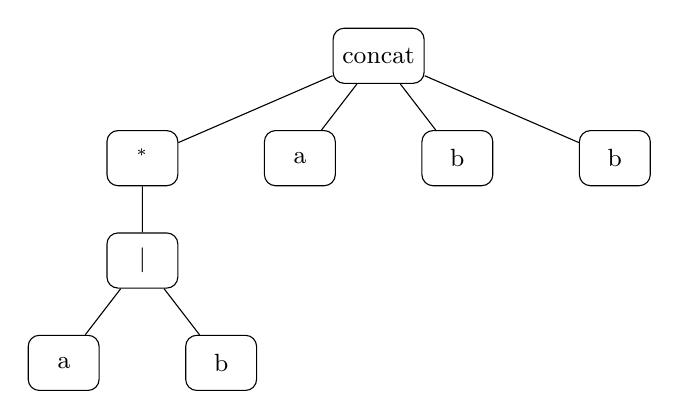
\begin{tikzpicture}[
  level distance=13mm,
  sibling distance=20mm,
  every node/.style={draw, rounded corners, minimum width=9mm, minimum height=7mm, align=center, font=\small}
]
\node {concat}
  child { node {$^{*}$}
    child { node {$\mid$}
      child { node {a} }
      child { node {b} }
    }
  }
  child { node {a} }
  child { node {b} }
  child { node {b} }
;
\end{tikzpicture}
\end{center}
\begin{center}
\small\textit{Syntax tree for $(a\mid b)^{*}abb$: the root concatenates four pieces --- the
starred union, then three literal symbols.}
\end{center}

\begin{examplebox}{Trace: Does \texttt{"babb"} Match?}
\texttt{babb} = \texttt{b} (matched by the $(a|b)^*$ part, one repetition) followed by
\texttt{a}, \texttt{b}, \texttt{b} (the literal suffix). Yes, it matches. Does \texttt{"abab"}
match? No -- it does not end in the literal substring \texttt{abb} (it ends in \texttt{bab}).
\end{examplebox}

\begin{examfocus}
Given an informal language description (``strings that start with \dots'', ``strings with an
even number of \dots'', ``strings that don't contain \dots''), be able to construct the regular
expression, and vice versa: given a regular expression, describe its language in English and
list 2--3 example strings it does and does not match. This two-way translation is the most
common exam pattern for this topic.
\end{examfocus}

\subsection{More Worked Examples}

\begin{center}
\renewcommand{\arraystretch}{1.4}
\begin{tabularx}{\textwidth}{@{}X l X@{}}
\toprule
\textbf{Language (in English)} & \textbf{Regular Expression} & \textbf{Matches / Doesn't Match} \\
\midrule
Binary strings with an even number of 0's & $1^{*}(01^{*}01^{*})^{*}$ & Matches \texttt{110011};
doesn't match \texttt{100} \\
Strings over $\{a,b\}$ containing at least one \texttt{a} & $(a\mid b)^{*}a(a\mid b)^{*}$ &
Matches \texttt{bba}; doesn't match \texttt{bbb} \\
Strings over $\{a,b\}$ \emph{not} containing the substring \texttt{aa} & $b^{*}(ab^{+})^{*}a^{?}$
& Matches \texttt{ababb}; doesn't match \texttt{baab} \\
C-style single-line comment & \texttt{//}$(\Sigma \setminus \{\text{newline}\})^{*}$ & Matches
\texttt{// TODO fix this}; doesn't match a two-line comment \\
\bottomrule
\end{tabularx}
\end{center}

\section{Regular Definitions}

\dbtag Writing out a complex regular expression as one giant unreadable formula is painful. A
\textbf{regular definition} lets us name intermediate regular expressions and reuse those names
in later definitions --- exactly like defining helper variables in ordinary algebra.

\begin{defbox}{Regular Definition}
A regular definition is a sequence $d_1 \to r_1,\ d_2 \to r_2,\ \dots,\ d_n \to r_n$ where each
$d_i$ is a new name, and each $r_i$ is a regular expression over $\Sigma \cup \{d_1,\dots,
d_{i-1}\}$ -- that is, $r_i$ may use the alphabet \emph{and} any name defined \emph{before} it,
but never itself or a later name (no recursive or forward references).
\end{defbox}

\subsection{Worked Example: Identifiers}

\begin{center}
\begin{tikzpicture}[
  box/.style={draw, thick, rounded corners, minimum height=0.9cm, minimum width=4.6cm, align=center, font=\small},
  >=Latex
]
  \node[box, fill=nuLight, draw=nuNavy] (letter) at (0,0) {\texttt{letter} $\to$ \texttt{a|b|}$\cdots$\texttt{|z|A|}$\cdots$\texttt{|Z}};
  \node[box, fill=nuLight, draw=nuNavy] (digit) at (0,-1.4) {\texttt{digit} $\to$ \texttt{0|1|}$\cdots$\texttt{|9}};
  \node[box, fill=dbGreenBg, draw=dbGreen] (id) at (7,-0.7) {\texttt{id} $\to$ \texttt{letter (letter|digit)*}};
  \draw[->, thick] (letter) -- (id);
  \draw[->, thick] (digit) -- (id);
\end{tikzpicture}
\end{center}

This is exactly $L(L\cup D)^{*}$ from the worked example in \S1.1, now written as a named,
reusable regular definition -- and it is the pattern for token \texttt{ID} in almost every
C-family language.

\subsection{Worked Example: Unsigned Numbers (DB's Classic Definition)}

Numbers like \texttt{5280}, \texttt{0.01}, \texttt{6.336E4}, or \texttt{1.89E-4} all need to be
matched by a single token pattern. DB builds this up from four named pieces:

\begin{center}
\begin{tikzpicture}[
  box/.style={draw, thick, rounded corners, minimum height=0.85cm, minimum width=5.3cm, align=center, font=\small},
  >=Latex
]
  \node[box, fill=nuLight, draw=nuNavy]  (digit)  at (0,0)    {\texttt{digit} $\to$ \texttt{0|1|}$\cdots$\texttt{|9}};
  \node[box, fill=nuLight, draw=nuNavy]  (digits) at (0,-1.3) {\texttt{digits} $\to$ \texttt{digit digit*}};
  \node[box, fill=enrichGoldBg, draw=enrichGold] (frac) at (0,-2.6) {\texttt{optionalFraction} $\to$ \texttt{.digits}\ $|\ \varepsilon$};
  \node[box, fill=enrichGoldBg, draw=enrichGold] (exp)  at (0,-3.9) {\texttt{optionalExponent} $\to$ \texttt{(E(+|-|}$\varepsilon$\texttt{)digits)}\ $|\ \varepsilon$};
  \node[box, fill=dbGreenBg, draw=dbGreen] (num) at (8.1,-1.95) {\texttt{num} $\to$\\ \texttt{digits optionalFraction}\\ \texttt{optionalExponent}};

  \draw[->, thick] (digit) -- (digits);
  \draw[->, thick] (digits.east) -- (num.west |- digits.east);
  \draw[->, thick] (frac.east) -- (num.west |- frac.east);
  \draw[->, thick] (exp.east) -- (num.west |- exp.east);
\end{tikzpicture}
\end{center}

\begin{examplebox}{Tracing \texttt{num} Against \texttt{6.336E4}}
\texttt{digits} matches \texttt{6}; \texttt{optionalFraction} matches \texttt{.336} (the
\texttt{.digits} branch); \texttt{optionalExponent} matches \texttt{E4} (the
$\varepsilon$-sign branch of \texttt{(E(+|-|}$\varepsilon$\texttt{)digits)}, since no
\texttt{+}/\texttt{-} appears). Concatenated: \texttt{6} + \texttt{.336} + \texttt{E4} =
\texttt{6.336E4}. For a plain integer like \texttt{5280}, both \texttt{optionalFraction} and
\texttt{optionalExponent} take their $\varepsilon$ branch and contribute nothing.
\end{examplebox}

\begin{examfocus}
Be able to reproduce this exact four-piece \texttt{num} definition from memory, and trace it
against a given number (integer, decimal, or scientific-notation) the way the example above
does. This is DB's single most frequently examined regular-definition example.
\end{examfocus}

\section{Extensions of Regular Expressions}

\beyonddb Modern regex notation (and DB \S3.3.5) adds a few extra operators. Formally, none of
these add any expressive power beyond plain union/concatenation/closure --- they are
\textbf{syntactic sugar}, purely for convenience and readability.

\begin{center}
\renewcommand{\arraystretch}{1.4}
\begin{tabularx}{\textwidth}{@{}l l X@{}}
\toprule
\textbf{Extension} & \textbf{Meaning} & \textbf{Equivalent to Core Regex} \\
\midrule
$r^{+}$ & one or more repetitions & $rr^{*}$ \\
$r^{?}$ & zero or one occurrence (optional) & $r \mid \varepsilon$ \\
$[abc]$ & character class: any one of \texttt{a}, \texttt{b}, \texttt{c} & $a \mid b \mid c$ \\
$[a\text{-}z]$ & character range: any letter from \texttt{a} to \texttt{z} & $a \mid b \mid
\cdots \mid z$ \\
$[\hat{}\,a]$ & negated class: any symbol \emph{except} \texttt{a} & union of all $x \in \Sigma
\setminus \{a\}$ \\
\bottomrule
\end{tabularx}
\end{center}

\begin{examfocus}
Know that $r^{+} \equiv rr^{*}$ and $r^{?} \equiv (r \mid \varepsilon)$ \emph{exactly} --- a
common trick question asks you to rewrite an extended-notation regex using only the three core
operators (union, concatenation, closure), which is precisely this substitution.
\end{examfocus}

\section{Regular vs.\ Non-Regular Languages}

\dbtag Not every language can be described by a regular expression. This matters enormously for
compiler design: it is exactly \emph{why} a single lexer pass is not enough, and why we need an
entirely different, more powerful formalism (context-free grammars, Lecture 8) for parsing.

\begin{coreidea}[The Central Limitation: No Counting]
A regular expression (equivalently, a finite automaton, Lectures 5--6) has no way to
\emph{count} an unbounded quantity and later check that count against something else. It can
verify local, bounded patterns, but it cannot verify \emph{global balance}. This single
limitation explains every classic example of a non-regular language.
\end{coreidea}

\begin{center}
\renewcommand{\arraystretch}{1.4}
\begin{tabularx}{\textwidth}{@{}X l X@{}}
\toprule
\textbf{Language} & \textbf{Regular?} & \textbf{Why} \\
\midrule
Identifiers: letter followed by letters/digits & \textbf{Yes} & Purely local: check each
character against a fixed small set of rules, no counting needed. \\
Fixed-format numeric literals & \textbf{Yes} & Same reason -- bounded structure, no unbounded
counting or matching required. \\
Balanced parentheses, e.g.\ $\{a^{n}b^{n} \mid n \ge 0\}$ & \textbf{No} & Requires counting how
many \texttt{(} were seen and demanding \emph{exactly} that many \texttt{)} later --- an
unbounded count with no fixed upper limit. \\
Matching HTML/XML open and close tags & \textbf{No} & Same reason, at the level of tags instead
of characters -- and worse, tags can \emph{nest}, requiring a stack, not just a counter. \\
Palindromes over $\{a,b\}$ & \textbf{No} & Requires comparing the first half of the string
against the reverse of the second half -- again, unbounded memory of what came before. \\
\bottomrule
\end{tabularx}
\end{center}

\begin{examplebox}{Why Finite Automata Can't Count: A Concrete Illustration}
Suppose you tried to build a finite automaton for balanced parentheses up to nesting depth $n$.
You would need at least one distinct state per depth level, $0, 1, 2, \dots, n$, just to
remember ``how many unmatched \texttt{(} have I seen so far.'' Since parentheses in real
programs can nest arbitrarily deep, no \emph{fixed, finite} number of states suffices for
\emph{every} possible program -- yet a finite automaton is required to have a fixed number of
states, decided in advance. This is the intuitive heart of the \textbf{pumping lemma for regular
languages} from your Automata Theory prerequisite: pump the middle of a long enough matched
string and you break the balance, proving no finite automaton can recognize it.
\end{examplebox}

\begin{takeaways}[Bridging Idea -- Why This Matters for the Rest of the Course]
\begin{itemize}
  \item Regular expressions/finite automata are the right tool for tokens: identifiers,
  numbers, keywords, operators -- all locally-checkable, bounded patterns.
  \item Nested and recursive structure -- matched parentheses, balanced braces, nested
  expressions, \texttt{if}/\texttt{else} matching -- is fundamentally \emph{beyond} what regular
  expressions can express, no matter how cleverly you write them.
  \item This is precisely why Lecture 8 introduces \textbf{context-free grammars}: a strictly
  more powerful formalism (using a stack, conceptually) that \emph{can} count and match nested
  structure, and precisely why the compiler needs \emph{two} separate formalisms --- one per
  phase --- instead of one universal one.
\end{itemize}
\end{takeaways}

\section{Beyond the Dragon Book: Regex in Practice}

\begin{enrichment}[Not All ``Regex'' Is Actually Regular]
This is a genuinely important and often-missed subtlety. Tools like Perl, Python's \texttt{re},
and JavaScript's regex support \textbf{backreferences} -- e.g.\ \texttt{(\textbackslash w+)
\textbackslash1} matches any word immediately repeated, like \texttt{hello hello}. This is
provably \emph{not} a regular language in the formal CS-theory sense used in this lecture ---
recognizing it requires comparing two substrings for equality, which needs unbounded memory,
just like the palindrome example above. Backreference-supporting engines use
\textbf{backtracking search}, not finite automata, under the hood; they are more accurately
called ``backtracking pattern matchers'' than true regular-expression engines. Meanwhile,
lexer-generator tools like Flex (Lecture 7) implement only \emph{true} regular expressions,
compiled to genuine finite automata, precisely because lexical analysis needs the speed and
predictability guarantees only real finite automata provide.
\end{enrichment}

\begin{enrichment}[Catastrophic Backtracking (ReDoS)]
Backtracking regex engines can, on adversarial input, take \emph{exponential} time on a pattern
that looks entirely innocent. The classic example is \verb|(a+)+b| applied to a long string of
\texttt{a}'s with no trailing \texttt{b}, like \texttt{"aaaaaaaaaaaaaaaaaaaaaaaaa!"}: the engine
tries exponentially many ways of splitting the a's between the inner and outer \texttt{+} before
giving up. This is a real, named security vulnerability class --- \textbf{ReDoS} (Regular
expression Denial of Service) --- and has caused real production outages (Cloudflare's July 2019
global outage was triggered by exactly this kind of catastrophic backtracking in a WAF rule).
The illustrative growth pattern:
\begin{center}
\small
\begin{tabular}{@{}lcccc@{}}
\toprule
Input length (a's, no trailing b) & 20 & 25 & 30 & 35 \\
\midrule
Illustrative matching steps (order of magnitude) & $\sim 10^5$ & $\sim 10^6$ & $\sim 10^8$ & $\sim 10^{10}$ \\
\bottomrule
\end{tabular}
\end{center}
This is exactly why the DFA-based matching you will learn in Lectures 5--6 -- which is
\emph{provably} linear in input length, with no possibility of this blow-up -- is not just a
theoretical nicety but the actual engineering reason production lexers never use a naive
backtracking matcher.
\end{enrichment}

\begin{enrichment}[Modern Guaranteed-Linear Engines]
Google's \textbf{RE2} library and Rust's \texttt{regex} crate deliberately give up
backreferences and a handful of other backtracking-only features specifically so that they can
guarantee linear-time matching via automata-based execution, immune to ReDoS by construction.
This is the industrial embodiment of the regular-vs-non-regular distinction from \S5: by
refusing to support genuinely non-regular features, these libraries buy back the performance
guarantee that true finite automata provide.
\end{enrichment}

\begin{enrichment}[Brzozowski Derivatives -- An Alternative to Automata]
Lectures 5--6 build a matcher for a regex by first converting it to a finite automaton (via
Thompson's construction). There is a completely different, more recent technique worth knowing
about: the \textbf{derivative} of a regular expression $r$ with respect to a symbol $a$,
written $\partial_a(r)$, is a new regular expression describing ``what still needs to match
after consuming an $a$.'' Repeatedly taking derivatives, one input symbol at a time, and
checking whether the final derivative accepts $\varepsilon$, matches a string \emph{without ever
building an explicit automaton at all}. Janusz Brzozowski introduced this in 1964; it fell out
of fashion for decades, then saw a resurgence starting around 2010 in functional-programming
circles (Scala's and Racket's parser-combinator libraries use derivative-based matching), because
derivatives compose beautifully with recursive data types in a way that hand-built automata do
not.
\end{enrichment}

\begin{enrichment}[Real-World Regex Flavors Differ]
The regex you type into \texttt{grep}, Python, or a Flex specification are not identical
languages -- they share the core ideas from this lecture but differ in surface syntax and
sometimes in power:
\begin{center}
\small
\renewcommand{\arraystretch}{1.3}
\begin{tabularx}{\textwidth}{@{}l X@{}}
\toprule
\textbf{Flavor} & \textbf{Notable differences} \\
\midrule
POSIX ERE (\texttt{grep -E}) & Closest to DB's formal core; no backreferences; character
classes like \texttt{[:digit:]}. \\
PCRE / Python \texttt{re} / JavaScript & Add backreferences, lookahead/lookbehind assertions,
non-greedy \texttt{*?}, named groups -- genuinely more expressive than regular languages. \\
Flex / lex specifications & Core regular expressions plus start conditions and direct
integration with symbol-table actions -- built to compile to a real DFA (Lecture 7). \\
\bottomrule
\end{tabularx}
\end{center}
Knowing which flavor you're targeting matters: a pattern copied from a Python script into a
Flex \texttt{.l} file may silently mean something different, or fail to compile at all.
\end{enrichment}

\section{Self-Check Questions}

\begin{enrichment}[Practice -- Not Graded]
\begin{enumerate}
  \item Write a regular expression for all strings over $\{0,1\}$ that \emph{start} with
  \texttt{1}. Then write one for strings that \emph{do not contain} the substring \texttt{00}.
  \item Using DB's \texttt{num} regular definition from \S3.2, trace the match for the literal
  \texttt{1.89E-4}, showing what each of \texttt{digits}, \texttt{optionalFraction}, and
  \texttt{optionalExponent} matches.
  \item Rewrite $r^{+}$ and $r^{?}$ using only union, concatenation, and Kleene closure (no
  extension operators allowed).
  \item Explain, in your own words and without using the word ``count,'' why balanced
  parentheses of arbitrary depth cannot be recognized by any regular expression.
  \item A teammate writes the regex \texttt{(a|aa)+b} and complains their program hangs on long
  inputs with no trailing \texttt{b}. What phenomenon is this, and why does it happen with a
  backtracking engine but not with a DFA-based one?
\end{enumerate}
\end{enrichment}

\begin{takeaways}
\begin{itemize}
  \item A language is just a set of strings; regular expressions are one \emph{notation} for
  describing certain languages, built inductively from $\varepsilon$, single symbols, union,
  concatenation, and Kleene closure.
  \item Precedence, highest to lowest: closure ($^{*}$), then concatenation, then union
  ($\mid$).
  \item \textbf{Regular definitions} let you name and reuse sub-expressions; DB's \texttt{id}
  and \texttt{num} definitions are the two canonical worked examples to know cold.
  \item Extension operators ($+$, $?$, character classes) add convenience, not expressive power
  -- each has an exact equivalent using only the three core operators.
  \item Regular expressions fundamentally \textbf{cannot count} an unbounded quantity, which is
  exactly why balanced parentheses, nested tags, and palindromes are \emph{not} regular -- and
  exactly why the compiler needs a second, more powerful formalism (context-free grammars) for
  parsing.
  \item Not everything called ``regex'' in practice is regular in the formal sense --
  backreference-supporting engines use backtracking and can suffer catastrophic (ReDoS)
  performance; true finite-automaton-based matching, which we build next, is immune to this by
  construction.
\end{itemize}
\end{takeaways}

\section*{References for This Lecture}
\begin{itemize}
  \item [DB] Aho, Lam, Sethi, Ullman. \textit{Compilers: Principles, Techniques, and Tools}, 2nd ed., \S3.3.
  \item [PP] Scott. \textit{Programming Language Pragmatics}, \S3.3.
\end{itemize}

\end{document}
